% Russian language
\documentclass{article}
\usepackage[utf8]{inputenc}
\usepackage[russian]{babel}

% Math symbols
\usepackage{amssymb}
\usepackage{amsmath}
\usepackage{accents}

% Images inplace
\usepackage{float}
\usepackage{graphicx}
% Code blocks
\DeclareFixedFont{\ttb}{T1}{txtt}{bx}{n}{8} % for bold
\DeclareFixedFont{\ttm}{T1}{txtt}{m}{n}{8}  % for normal
\usepackage{color}
\definecolor{deepblue}{rgb}{0,0,0.5}
\definecolor{deepred}{rgb}{0.6,0,0}
\definecolor{deepgreen}{rgb}{0,0.5,0}
\usepackage{listings}
\newcommand\pythonstyle{\lstset{
language=Python,
basicstyle=\ttm,
morekeywords={self},              % Add keywords here
keywordstyle=\ttb\color{deepblue},
emph={MyClass,__init__},          % Custom highlighting
emphstyle=\ttb\color{deepred},    % Custom highlighting style
stringstyle=\color{deepgreen},
frame=tb,                         % Any extra options here
showstringspaces=false
}}
\lstnewenvironment{python}[1][]
{
\pythonstyle
\lstset{#1}
}
{}
\newcommand\pythonexternal[2][]{{
\pythonstyle
\lstinputlisting[#1]{#2}}}
\newcommand\pythoninline[1]{{\pythonstyle\lstinline!#1!}}
% Code blocks

\makeatletter
\renewcommand*\env@matrix[1][*\c@MaxMatrixCols c]{%
  \hskip -\arraycolsep
  \let\@ifnextchar\new@ifnextchar
  \array{#1}}
\makeatother

\title{Лабораторная работа №1}
\author{Ларин Егор. 4 группа 3 курс}

\begin{document}
\maketitle
\section*{Теория}
\subsection*{Задача}
\begin{equation*}
    u'' = 2x + 2 - 2xu' + 4 u
\end{equation*}

$$\begin{cases}
    u'(0) = -1\\
    u'(1) = 1 - 2u(1)
\end{cases}$$

\subsection*{Разностная схема}

\begin{equation*}
    u_{\overline{x}x} = \frac{u(x+h) - 2u(x) + u(x-h)}{h^2}
\end{equation*}

\begin{equation*}
    u_{\mathring{x}} = \frac{u(x+h) - u(x-h)}{2h}
\end{equation*}

$$y_{\overline{x}x} = 2 x + 2 - 2x u_{\mathring{x}} + 4u$$

$$y(x-h) \left(\frac{1}{h^2} - \frac{x}{h}\right) + y(x) \left(\frac{-2}{h^2} - 4\right) + y(x+h) \left(\frac{1}{h^2} + \frac{x}{h}\right) = 2x + 2$$
$$y_{i-1} \left(\frac{1}{h^2} - \frac{x_i}{h}\right) + y_i \left(\frac{-2}{h^2} - 4\right) + y_{i+1} \left(\frac{1}{h^2} + \frac{x_i}{h}\right) = 2x + 2, i = \overline{1, N-1}$$ 

$$y_1 + y_0 \left(-1 +2h^2\right) = -h + h^2$$
$$y_N \left(1 + 2h + 4h^2\right) - y_{N-1} = h - h^2$$



\section*{Листинг кода}
\begin{python}
from math import ceil
import numpy as np
from matplotlib import pyplot as plt

def TDMA(a, b, c, d):
    n = len(d)
    w= np.zeros(n-1,float)
    g= np.zeros(n, float)
    p = np.zeros(n,float)
    
    w[0] = c[0]/b[0]
    g[0] = d[0]/b[0]

    for i in range(1,n-1):
        w[i] = c[i]/(b[i] - a[i-1]*w[i-1])
    for i in range(1,n):
        g[i] = (d[i] - a[i-1]*g[i-1])/(b[i] - a[i-1]*w[i-1])
    p[n-1] = g[n-1]
    for i in range(n-1,0,-1):
        p[i-1] = g[i-1] - w[i-1]*p[i]
    return p

def u(x):
    return x**2 - x

def solve(h):
    # c lower
    # a middle
    # b upper

    N = ceil(1 / h)

    b_1 = [1] ##
    b_i = [1 + (i*h) * h for i in range(1,N)] #

    a_1 = [2*h**2 - 1] ##
    a_i = [-2 - 4 * h**2 for i in range(1, N)] #
    a_N = [1 + 2 *h +4*h**2]

    c_i = [1 - (i*h)*h for i in range(1, N)] #
    c_N = [-1]
    
    f_1 = [-h+h**2] ##
    f_i = [(2*(i*h) + 2) * h**2 for i in range(1, N)] #
    f_N = [h-h**2]

    ys = TDMA(
        c_i + c_N,
        a_1 + a_i + a_N,
        b_1 + b_i,
        f_1 + f_i + f_N,
    )

    xs = [i * h for i in range(N+1)]
    plt.plot(xs, ys, "ro", xs, [u(x) for x in xs], "b")
    plt.legend(["$y(x)$", "$u(x)$"])
    plt.show()

    print(ys)
    print(max([u(x) - y for (x,y) in zip(xs, ys)]))
    return ys



y1 = solve(0.02)
y2 = solve(0.01)
print(max([abs(y2[2*i] - y1[i]) for i in range(ceil(1 / 0.02))]))




\end{python}

\section*{Графики}
\begin{figure}[H]
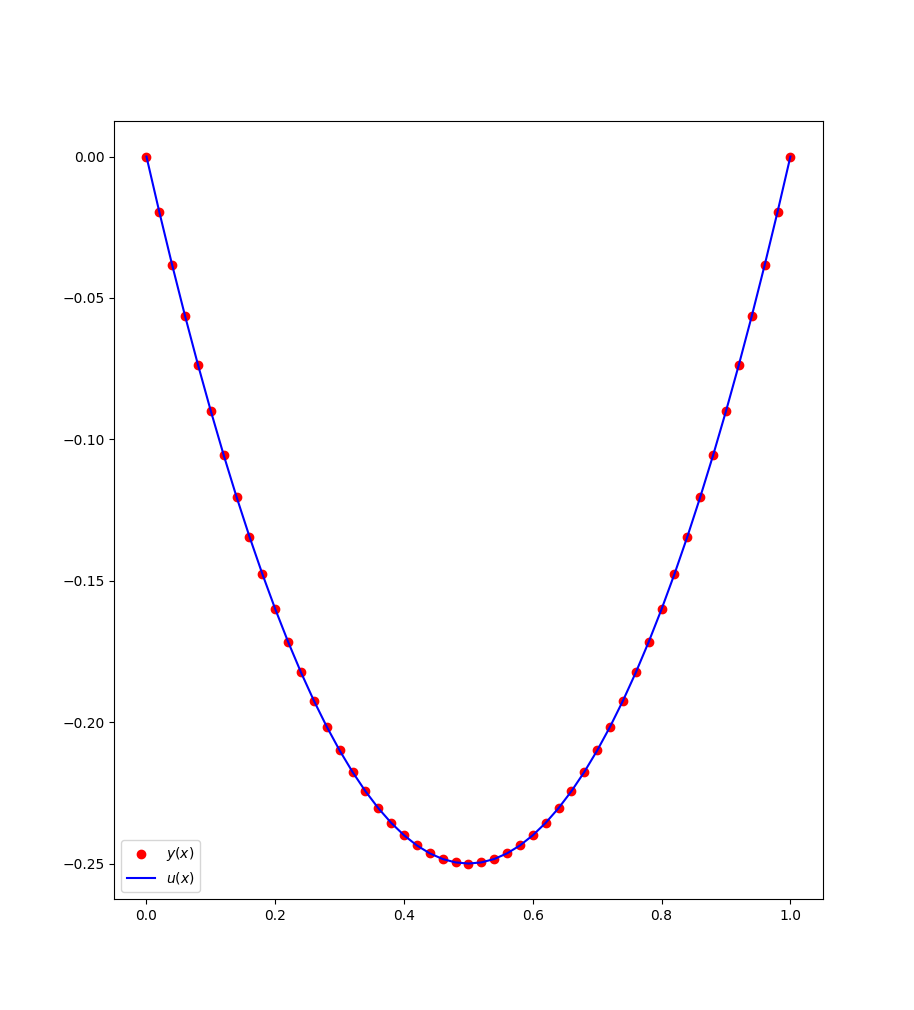
\includegraphics[width=0.5\textwidth]{Figure_1.png}
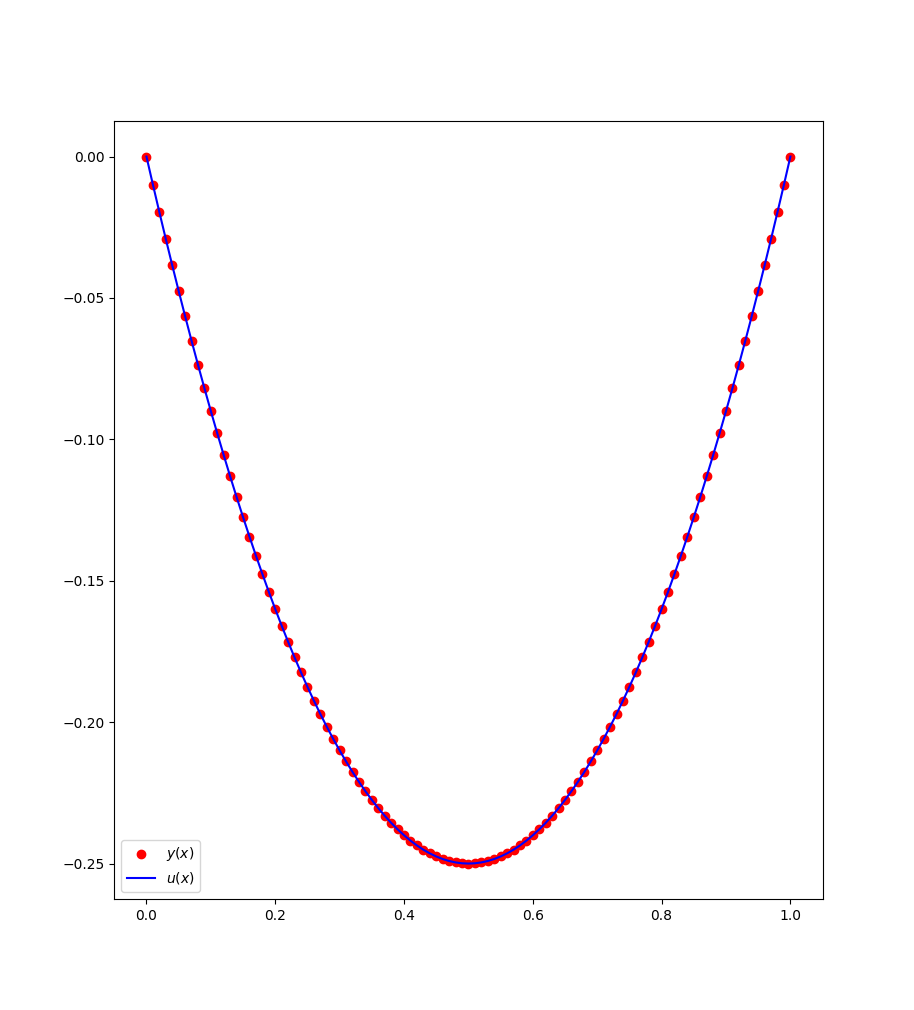
\includegraphics[width=0.5\textwidth]{Figure_2.png}
\end{figure}

\section*{Результаты вычислительного эксперимента}
\begin{tabular}[H]{|l|l|}
  \hline
  Величина & Погрешность \\
  \hline
  $y_{h}$ &  1.6681100944992977e-14 \\
  $y_{\frac{h}{2}}$ &  1.4016565685892601e-14  \\
  $\frac{1}{3} \max \left|y^h - y^{\frac{h}{2}}\right|_{\omega_h}$ & 2.8727020762175925e-15 \\
  \hline
\end{tabular} 
\end{document}
